\documentclass{ximera}

%\addPrintStyle{..}

\begin{document}
	\author{Bart Lambregs}
	\xmtitle{Vraagstukken}{}
    \xmsource\xmuitleg

\begin{exercise}
    Een automobilist rijdt op een rechte baan gedurende \SI{1,5}{\hour} aan \SI{80}{\kilo\meter\per\hour} en daarna gedurende dezelfde tijdsduur aan
    \SI{70}{\kilo\meter\per\hour} in dezelfde zin.
    \begin{question} 
        Wat is zijn gemiddelde snelheid?
        \begin{oplossing}
            \(\overline{v} = \frac{\Delta x_{\text{tot}}}{t_{\text{tot}}} = \frac{\Delta x_1 + \Delta x_2}{\Delta t_1 + \Delta t_2} = \frac{v_1 \cdot \Delta t_1 + v_2 \cdot \Delta t_2}{\Delta t_1 + \Delta t_2} = \SI{75}{\km\per\hour}\)
        \end{oplossing}
    \end{question}

    \begin{question} 
        Met welke snelheid had hij moeten rijden om met een constante snelheid hetzelfde traject in dezelfde tijd af te leggen? 
        \begin{oplossing}
            \SI{75}{\km\per\hour}
        \end{oplossing}
    \end{question}
\end{exercise}

\begin{exercise}
    Een fietser legt een bepaalde afstand af over een zekere tijd. Gedurende de eerste helft van de tijd houdt hij constant een snelheid $v_1$ aan, gedurende de tweede helft een snelheid $v_2$. Wat is zijn gemiddelde snelheid over het totale tijdsinterval?
    \begin{oplossing}
        \(\overline{v} = \frac{\Delta x_{\text{tot}}}{t_{\text{tot}}} = \frac{\Delta x_1 + \Delta x_2}{\Delta t_1 + \Delta t_2} = \frac{v_1 \cdot \Delta t_1 + v_2 \cdot \Delta t_2}{\Delta t_1 + \Delta t_2} = \frac{v_1 \cdot \frac{\Delta t_{\text{tot}}}{2} + v_2 \cdot \frac{\Delta t_{\text{tot}}}{2}}{\Delta t_{\text{tot}}} =\frac{v_1+v_2}{2} \)
    \end{oplossing}
\end{exercise}

\begin{exercise}
    Een automobilist legt \SI{120}{km} af. De eerste helft van de weg legt hij af aan \SI{90}{\kilo\meter\per\hour}, de tweede helft aan \SI{120}{\kilo\meter\per\hour}. Wat is zijn gemiddelde snelheid?
    \begin{oplossing}
        \(\overline{v} = \frac{\Delta x_{\text{tot}}}{t_{\text{tot}}} = \frac{\Delta x_1 + \Delta x_2}{\Delta t_1 + \Delta t_2} =  \frac{\Delta x_1 + \Delta x_2}{\frac{\Delta x_1}{v_1} + \frac{\Delta x_2}{v_2}} = \frac{\Delta x_{\text{tot}}}{\frac{\Delta x_{\text{tot}}}{v_1} + \frac{\Delta x_{\text{tot}}}{v_2}} = \frac{2\cdot v_1 \cdot v_2}{v_1 + v_2} = \SI{103}{\km\per\hour} \)
    \end{oplossing}
\end{exercise}

\begin{exercise}
    Een fietser legt een bepaalde afstand af over een zekere tijd. Gedurende de eerste helft van de af te leggen afstand houdt hij constant een snelheid $v_1$ aan, gedurende de tweede helft een snelheid $v_2$. Wat is zijn gemiddelde snelheid over het totale tijdsinterval? 
\begin{oplossing}
  $\overline{v}=\frac{2v_1v_2}{v_1+v_2}$
\end{oplossing}
\end{exercise}

\begin{exercise}
    Als je met de fiets heen en terug naar school rijdt en in het heengaan tegenwind en in het terugkeren rugwind hebt, compenseert dat dan mekaar precies?

    Stel om dit op te lossen dat de weg rechtlijnig is. Bereken je gemiddelde snelheid over het traject heen en terug en vergelijk die met de snelheid die je zonder wind zou halen. Neem aan dat je normaal \SI{20}{\kilo\meter\per\hour} zou fietsen, maar door de wind win of verlies je \SI{2}{\kilo\meter\per\hour}.
    \begin{multipleChoice}
        \choice[correct]{Nee, je hebt netto een nadeel vanwege de tegenwind.}
        \choice{Nee, je hebt netto een voordeel vanwege de rugwind.}
        \choice{Ja, de afstand heen is de afstand terug, dus het is net alsof je helemaal geen wind had.}
    \end{multipleChoice}
    \begin{feedback}
    Zie vorige opgaves. Omdat je in tijd langer de trage snelheid aanhoudt, zal de gemiddelde snelheid dichter bij de trage snelheid liggen. 
    \end{feedback}
\end{exercise}

\begin{exercise}
    Een bowlingbal die met een constante snelheid voortrolt, raakt de kegels aan het einde van een kegelbaan van \SI{16,5}{m} lengte. De werper hoorde het geluid waarmee de bal op de kegels botst \SI{2,5}{s} nadat hij de bal losliet. Welke snelheid had de bal? De snelheid van het geluid is \SI{343}{m/s}. 
    \begin{oplossing}
        $ \Delta t_{\text{tot}} = \Delta t_1 + \Delta t_2 = \frac{\Delta x}{v_1} + \frac{\Delta x}{v_2} \Rightarrow v_1=\frac{x_1}{t_2-\frac{x_1}{v_2}}=\SI{6,73}{m/s}$
    \end{oplossing}
\end{exercise}

\begin{exercise}
    Een vliegtuig moet minstens een snelheid van \SI{108}{\kilo\meter\per\hour} hebben om te kunnen opstijgen. Indien de propellers aan het toestel een versnelling van \SI{1,50}{m/s^2} geven, hoe lang moet de startbaan dan minstens zijn? 
    \begin{oplossing}
    % \item[gegeven]$v=30,0\rm\,m/s$\newline$a=1,50\rm\,m/s^2$
    % \item[gevraagd]$x$
    % \item[oplossing]
    Doordat we de versnelling van het vliegtuig kennen en de snelheid die het moet bereiken, kunnen we de tijd die het vliegtuig hiervoor nodig heeft, gemakkelijke berekenen met de formule $v=v_0+at$ voor de snelheid van een EVRB:
    \begin{eqnarray*}
        t=\frac{v}{a}
    \end{eqnarray*}
    De afstand die in deze tijd wordt afgelegd, kunnen we berekenen doordat we de gemiddelde snelheid kennen\footnote{De benodigde afstand kunnen we evenzeer berekenen met de formule $x=x_0+v_0+\frac{1}{2}at^2$ door de tijd in te vullen.}:
    \begin{eqnarray*}
    x&=&\frac{v_0+v}{2}\cdot t\\
    &=&\frac{v}{2}\cdot\frac{v}{a}\\
    &=&\frac{v^2}{2a}
    \end{eqnarray*}
    De startbaan moet dus minstens \SI{300}{m} lang zijn.
    \end{oplossing}
\end{exercise}

\begin{exercise}
    Een trein rijdt aan een snelheid van \SI{72}{\kilo\meter\per\hour} en remt met een versnelling waarvan de grootte \SI{1,0}{m/s^2} bedraagt. Na hoeveel tijd komt de trein tot stilstand en welke afstand wordt er tijdens dit afremmen afgelegd?

    \begin{oplossing}
        % \item[gegeven]$v_0=\SI{20}{m/s}\newline $a=\SI{-1,0}{m/s^2}
        % \item[gevraagd]$t$, $x$
        % \item[oplossing]
        Aangezien er per seconde een snelheid van \SI{1,0}{m/s} van de beginsnelheid afgaat, vinden we de tijd die nodig is voor het remmen, door de beginsnelheid te delen door de versnelling. Dat is namelijk de tijd die nodig is voor de trein om tot stilstand te komen:
        \begin{eqnarray*}
            v&=&0\\
            &\Updownarrow&\\
            v_0+at&=&0\\
            &\Updownarrow&\\
            t&=&-\frac{v_0}{a}
        \end{eqnarray*}
        Invullen van de gegevens levert een tijd van \SI{20}{s}. De afgelegde afstand gedurende het remmen vinden we nu met de plaatsfunctie. We kennen de benodigde tijd, die we in de plaatsfunctie invullen.
        \begin{eqnarray*}
            x&=&v_0t+\frac{1}{2}at^2\\
            &=&v_0\left(-\frac{v_0}{a}\right)+\frac{1}{2}a\left(-\frac{v_0}{a}\right)^2\\
            &=&-\frac{v_0^2}{a}+\frac{v_0^2}{2a}\\
            &=&-\frac{v_0^2}{2a}\\
        \end{eqnarray*}
        Invullen van de gegevens levert een remafstand van \SI{200}{m}. 

        Een andere mogelijkheid om de remafstand te vinden is te werken met de gemiddelde snelheid, $x=\overline{v}t$.
    \end{oplossing}
\end{exercise}

\begin{exercise}
    Op een bevroren meer komt een glijdende hockeyschijf na \SI{200}{m} tot stilstand. Als zijn initi\"ele snelheid \SI{3,00}{m/s} was, bepaal dan
    \begin{question} Bepaal de versnelling in de veronderstelling dat deze constant is. 
        \begin{oplossing} 
        Er is gegeven dat: 
        \begin{itemize}
            \item \(\Delta x = \SI{200}{\meter}\)
            \item \(v_0 = \SI{3}{\meter\per\second}\)
            \item \(v_1 = \SI{0}{\meter\per\second}\)
        \end{itemize}
        Omdat de beweging een EVRB is geldt \(\overline{v} = \frac{v_0 + v_1}{2}\) In het algemeen geldt ook \(\overline{v} = \frac{\Delta x}{\Delta t}\). Uit deze gelijkheden halen we \(\Delta t = \frac{2\Delta x}{v_1}\). Hiermee kan de versnelling van de EVRB bepaald worden: 
        $a= \overline{a} = \frac{\Delta v}{\Delta t} = \frac{v_1 - v_0}{\Delta t}=\SI{0.0225}{\meter\per\second\squared}$;    
        \end{oplossing} 
    \end{question}
    
    \begin{question} Bepaal de tijd die de schijf nodig heeft om tot stilstand te komen. 
    \begin{oplossing} 
    Uit de vorige deelvraag halen we dat $t=\frac{2x}{v_0}=\SI{133,33}{s}$                                
    \end{oplossing} 
    \end{question}

\end{exercise}

\begin{exercise}
    Een bootje vaart met een snelheid van \SI{36,0}{\kilo\meter\per\hour} een eerste tijdopnemer voorbij en drijft daarna eenparig zijn snelheid op. Na \SI{20,0}{\second} komt het voorbij een tweede tijdopnemer met een snelheid van \SI{90,0}{\kilo\meter\per\hour}. Bereken de versnelling van het bootje en de afstand tussen beide tijdopnemers.
    \begin{oplossing}
    De beweging is een EVRB, er geldt $a= \overline{a} = \frac{v-v_0}{t-t_0}= \frac{\SI{25}{\meter\per\second} - \SI{10}{\meter\per\second}}{\SI{20}{\second}} = \SI{0,750}{\meter\per\second\squared} $
        
        
    De afstand vinden we met $x-x_0=\left(\frac{v_0+v}{2}\right)(t-t_0)=\SI{350}{m}$
    \end{oplossing}
\end{exercise}

\begin{exercise}
    Een auto vertrekt vanuit rust en bereikt na \SI{3,0}{km} een snelheid van \SI{450}{\kilo\meter\per\hour} We onderstellen de versnelling constant en de baan recht. Bereken de versnelling en de tijd, nodig om die \SI{3,0}{km} af te leggen.
\begin{oplossing}
    Er is gegeven dat 
    \begin{itemize}
        \item \( \Delta x  = \SI{3000}{\meter}\)
        \item \(v_0 = 0\)
        \item \(v_1 = \SI{125}{\meter\per\second}\)
    \end{itemize}

    Omdat voor een EVRB de gemiddelde snelheid gegeven wordt door $\overline{v}=\frac{v_0+v}{2}$ en we de afgelegde afstand kennen, kunnen we de benodigde tijd gemakkelijk vinden. We kiezen $t_0=0$, $x_0=0$. De beginsnelheid is nul zodat:
    \begin{eqnarray*}
        \Delta x &=& \overline{v}\Delta t \\
        &\Downarrow & \\
        t &=& \frac{x}{\left(\frac{v}{2}\right)} = \frac{2x}{v}
    \end{eqnarray*}
    Invullen van de gegevens levert een tijd van \SI{48}{s}. Met de formule $v=v_0+at$ voor de snelheid vinden we de versnelling door de tijd erin te substitueren, en de beginsnelheid nul te nemen:
    \begin{eqnarray*}
        % v &=& at \\
        % &\Updownarrow&\\
        a &=& \frac{v}{t}=\frac{v}{\left(\frac{2x}{v}\right)}\\
        &=& \frac{v^2}{2x}
    \end{eqnarray*}
    Invullen van de gegeven grootheden levert een versnelling van \SI{2,6}{m/s^2}.
\end{oplossing}
\end{exercise}

\begin{exercise}
    Een auto begint te remmen als hij zich \SI{35}{m} van een stilstaande hindernis bevindt. Zijn snelheid op dat moment is \SI{54}{\kilo\meter\per\hour}. Na \SI{4,0}{s} botst hij tegen de hindernis. Bereken de snelheid waarmee hij de hindernis raakt en zijn constante versnelling gedurende de remweg.
    \begin{oplossing}
    Uit de plaatsfunctie $x=v_0t+\frac{1}{2}at^2$ kunnen we de versnelling halen:
    \begin{equation*}
        a=\frac{2x-2v_0t}{t^2}=\SI{-3,125}{m/s^2}
    \end{equation*}
    Substitutie van de versnelling in de snelheidsfunctie levert:
    \begin{eqnarray*}
        v&=&v_0+at\\
        &=&v_0+\left(\frac{2x-2v_0t}{t^2}\right)t\\
        &=&\frac{2x}{t}-v_0\\
        &=&\SI{2,5}{m/s}
    \end{eqnarray*}
    Een andere (snellere) mogelijkheid om de snelheid te vinden is die te halen uit $x=\frac{v_0+v}{2}t$.
    \end{oplossing}
\end{exercise}

\begin{exercise}
    Twee fietsers vertrekken gelijktijdig om een afstand van \SI{200}{m} af te leggen. De eerste rijdt met een constante snelheid van \SI{4,0}{m/s}, terwijl de tweede vertrekt met een snelheid van \SI{1,00}{m/s} en de afstand van \SI{200}{m} met een EVRB met een versnelling van \SI{0,20}{m/s^2} aflegt. Waar zal de tweede fietser de eerste inhalen en wanneer?
    \begin{oplossing}
    Er is gegeven: 
    \begin{itemize}
        \item \(\Delta x = \SI{200}{\meter}\)
        \item \(x_{o,A} = x_{0,B} = 0\)
        \item \(v_A = \SI{4}{\meter\per\second}\)
        \item \(v_{0,B} = \SI{1}{\meter\per\second}\)
        \item \(a_B = \SI{0,20}{\meter\per\second\squared}\)
    \end{itemize}

    Fietser A beweegt volgens een ERB met voorschrift \(x_A = x_{0,A} + v_A t = v_a  t\). \\

    Fietsen B begeegt volgens een ECRB met voorschrift \(x_B = x_{0,B} + v_{0,B} t + \frac{1}{2} a_B t^2 = v_{0,B} t + \frac{1}{2} a_B t^2 \)

    De plaatsfuncites aan elkaar gelijkstellen levert: 
    \[
    \begin{array}{rcl}
        x_A &=& x_B \\ 
        &\Downarrow& \\
        v_A t &=& v_{0,B}t + \frac{1}{2}a_B t^2\\
        &\Downarrow& \\
        \frac{1}{2}a_b t^2 + (v_{0,B} - V_A)t &=& 0 \\
        &\Downarrow& \\
        t\left( \frac{1}{2}a_Bt + v_{0,B} - v_A \right) &=& 0
    \end{array}
    \]
    De oplossing \(t_0 = 0\) is triviaal aangezien ze samen vertrekken. De andere factor is nul indien: 

    \[
    \begin{array}{rcl}
        \frac{1}{2}a_Bt&=& v_A-V_{0,B} \\
        &\Downarrow& \\
        t_1 &=& \frac{2{v_A - v_{0,B}}}{a_B} = \SI{30}{\second}
    \end{array}\]


    Invullen levert als oplossing $x=v_At=\frac{2v_A(v_A-v_{B,0})}{a}=\SI{120}{m}$
    \end{oplossing}

\end{exercise}

\begin{exercise}
        Een trein vertrekt om 12u00 in het station a en rijdt naar het station b, op \SI{15}{\kilo\meter} van a gelegen. 
        De eerste \SI{1000}{\meter} worden afgelegd met een EVRB en de verkregen snelheid is \SI{72}{\kilo\meter\per\hour}. 
        Die snelheid blijft constant tot op \SI{250}{\meter} van b. Hier begint de trein te vertragen. Om hoe laat komt de trein in station b toe? Maak de $v(t)$-grafiek.

        \begin{oplossing}
        We maken eerst een grafiek van het traject van de trein: 
        \begin{image}
            
            \begin{tikzpicture}
                \draw[->] (0, -0.5) --  (0,5) node[above]{$v$};
                \draw[->] (-0.5, 0) -- (6,0) node[right]{$t$};
                
                \draw (0,0) -- node[midway, above left]{EVRB} (2, 4) -- node[midway, above]{ERB} (4, 4) -- node[midway, above right]{EVRB} (5, 0); 
                
                \draw[dotted] (2,4) -- (2, 0) node[below]{$t_1$}; 
                \draw[dotted] (4,4) -- (4, 0) node[below]{$t_2$}; 
            \end{tikzpicture}
        \end{image}
        Er is gegeven dat 
        \begin{itemize}
            \item \(v_0 = 0\)
            \item \(v_2 = \SI{20}{\meter\per\second}\)
            \item \(v_e = 0\)
        \end{itemize}

        Er geldt
        \renewcommand{\arraystretch}{2.5}
        \[
        \begin{array}{rcl}
        \Delta t &=& \Delta t_1 + \Delta t_2 + \Delta t_3 \\
        &=& \frac{\Delta x_1}{\overline{v}_1} + \frac{\Delta x_2}{\overline{v}_2} + \frac{\Delta x_3}{\overline{v}_3}\\
        &=& \frac{\Delta x_1}{\frac{v_0 + v_2}{2}} + \frac{\Delta x_2}{v_2} + \frac{\Delta x_3}{\frac{v_2 + v_e}{2}}\\
        &=& \frac{2\Delta x_1}{\overline{v}_1} + \frac{\Delta x_2}{v_2} + \frac{2\Delta x_3}{v_2}\\
        &=& \frac{2 \cdot \SI{1000}{\meter}}{\SI{20}{\meter\per\second}} + \frac{\SI{15000}{\meter} - \SI{1000}{\meter} - \SI{250}{\meter}}{\SI{20}{\meter\per\second}} + \frac{2\cdot \SI{250}{\meter}}{\SI{20}{\meter\per\second}}\\
        &=& \SI{100}{\second} + \SI{687.5}{\second} + \SI{25}{\second}\\ 
        &=& \SI{813}{\second}
        \end{array} 
        \]
        \renewcommand{\arraystretch}{1}


        % \SI{813}{\second} komt overeen met \(13\) minuten en \SI{33}{\second}. 
        De trein komt aan om \(12\)u\(12\)m\(33\)s

        \end{oplossing}
\end{exercise}

\begin{exercise}
    Een deeltje beschrijft een eendimensionale beweging op de $x$-as. De positie als functie van de tijd is hiernaast weergegeven in een $x(t)$-diagram. Duid de onderstaande grafiek aan die het best het verloop weergeeft van de snelheidscomponent $v$ van dat deeltje als functie van de tijd. 

    \begin{image}
        \begin{tikzpicture}[scale=1]
            % Axes
            \draw[->,thick] (0,0) -- (5,0) node[below right] {$t$};
            \draw[->,thick] (0,0) -- (0,5) node[left] {$x$};
            \filldraw (0,0) circle (2pt);
          
            % Curve (parabola-like)
            \draw[thick,domain=0:4,smooth,variable=\t] 
                 plot ({\t}, {0.3*(\t-1)^2 + 1});
          
            % Label at origin
            \node[below left] at (0,0) {O};
          \end{tikzpicture}
    \end{image}
    \captionof{figure}{De grafiek van de plaatsfunctie $x(t)$-diagram}

    % \begin{image}
    %     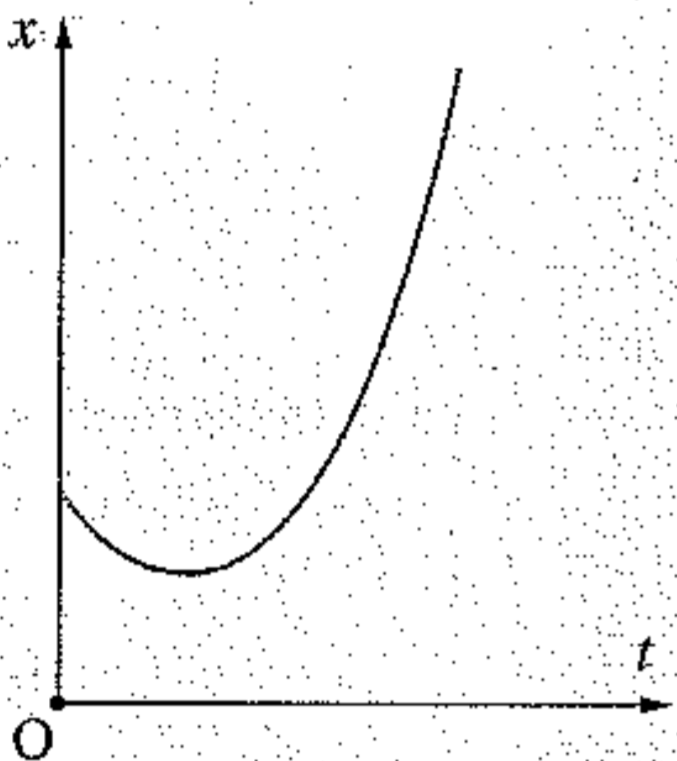
\includegraphics[width=\textwidth]{snelheidsverloop_o}
    % \end{image}


\begin{image}
    \begin{tikzpicture}

		\begin{scope}[shift={(0,0)}]
		  \draw[->] (0,0) -- (3.5,0) node[below right] {$t$};
		  \draw[->] (0,-2) -- (0,2.5) node[left] {$v_x$};
		  \fill (0,0) circle (1.2pt) node[left] {O};

          \draw[thick] (0,-1.5) -- (3,2);
		\end{scope}
		
		\begin{scope}[shift={(5,0)}]
		  \draw[->] (0,0) -- (3.5,0) node[below right] {$t$};
		  \draw[->] (0,-0.5) -- (0,2.5) node[left] {$v_x$};
		  \fill (0,0) circle (1.2pt) node[left] {O};

          \draw[thick] (0,1) -- (3,2);
		\end{scope}
		
		\begin{scope}[shift={(10,0)}]
		  \draw[->] (0,0) -- (3.5,0) node[below right] {$t$};
		  \draw[->] (0,-2) -- (0,2.5) node[left] {$v_x$};
		  \fill (0,0) circle (1.2pt) node[left] {O};

          \draw[thick,domain=0:3,smooth,variable=\t] plot ({\t},{1.2*sin(120*\t)});
		\end{scope}
		
		\begin{scope}[shift={(15,0)}]
		  \draw[->] (0,0) -- (3.5,0) node[below right] {$t$};
		  \draw[->] (0,-2) -- (0,2.5) node[left] {$v_x$};
		  \fill (0,0) circle (1.2pt) node[left] {O};

          \draw[thick] (0,1.5) -- (3,-1.5);
		\end{scope}
		
	\end{tikzpicture}
\end{image}

\begin{oplossing}
    Grafiek A 
\end{oplossing}

    % \begin{image}
    %     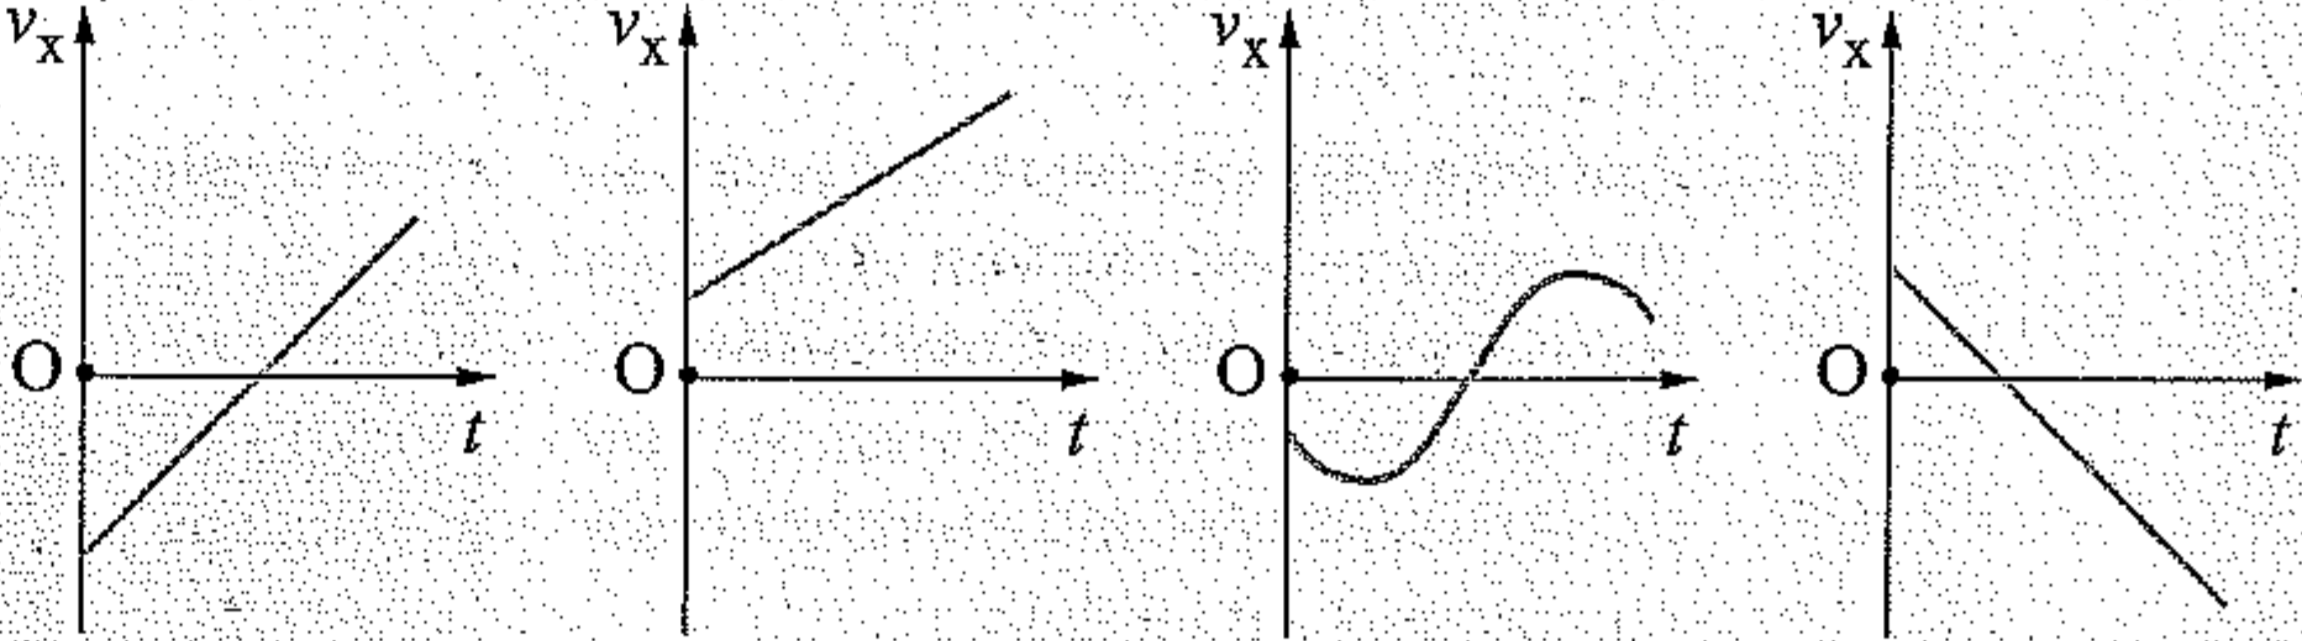
\includegraphics[width=0.93\textwidth]{snelheidsverloop}
    % \end{image}
\end{exercise}

\begin{exercise}
Een deeltje beweegt in de zin van de $x$-as. De onderstaande grafiek geeft aan hoe de grootte van de snelheid verandert als functie van de tijd.
\begin{image}
    \begin{tikzpicture}[xscale=0.5]
        \draw[->] (0,0) -- (32,0) node[right, font=\Large] {$t$ (s)};
        \draw[->] (0,0) -- (0,13) node[above, font=\Large] {$v$ (m/s)};
        
        \draw[dashed] (0,12) -- (5,12);
        \draw[dashed] (5,0) -- (5,12);
        \draw[dashed] (15,0) -- (15,12);
        
        \foreach \x in {0,5,15,30}
            \draw (\x,0) -- (\x,-0.2) node[below] {\x};
        \foreach \y in {4,8,12}
            \draw (0,\y) -- (-0.2,\y) node[left] {\y};
        
        \draw[thick] (0,0) -- (5,12) -- (15,12) -- (30,0);
    \end{tikzpicture}	
    \end{image}
    \captionof{figure}{snelheidsfunctie}


% preTikz... 
% \begin{image}
%     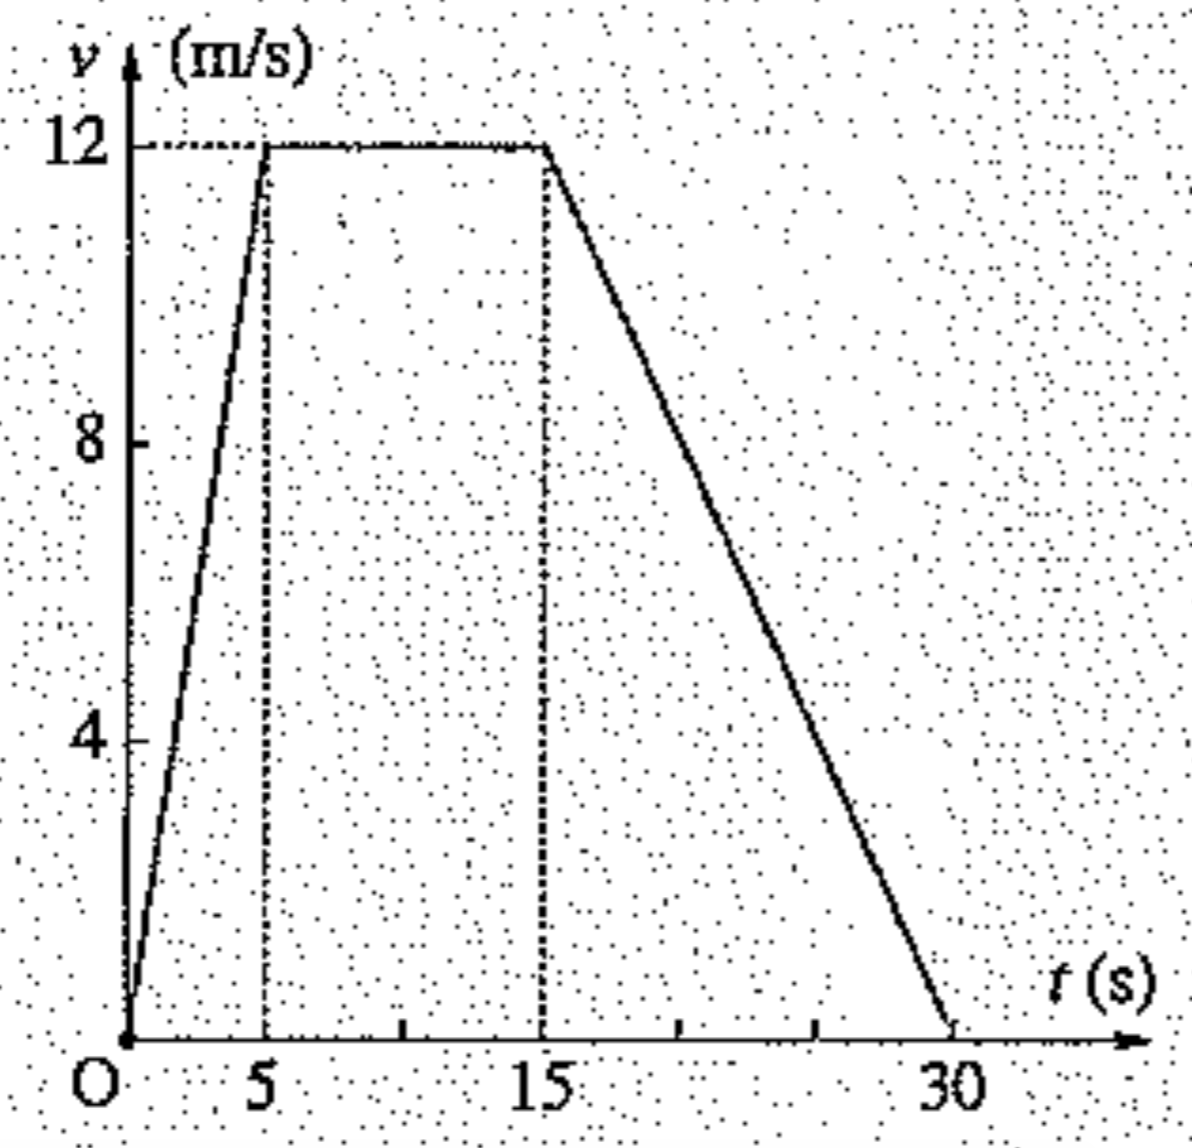
\includegraphics[width=\textwidth]{snelheidsverloop_2_o}
% \end{image}

\begin{question}
De afstand afgelegd na \SI{15}{s} bedraagt:
\wordChoice{
    \choice{\SI{30}{\meter}}
    \choice{\SI{120}{\meter}}
    \choice[correct]{\SI{150}{\meter}}
    \choice{\SI{240}{\meter}}
}
\begin{feedback}
    \(\Delta x = \Delta x_1 + \Delta x_2  = \overline{v}_1\cdot \Delta t_1 + v_2\cdot \Delta t_2 = \frac{v_0 + v_1}{2} \cdot \Delta t_1 + v_2 \delta t_2 = \SI{30}{\meter} + SI{120}{\meter} = \SI{150}{\meter}\)
\end{feedback}
\end{question}

\begin{question}
Na \SI{30}{s} heeft het deeltje een welbepaalde afstand afgelegd. Hoe groot zou de constante snelheid van het deeltje moeten zijn om in \SI{30}{s} dezelfde afstand af te leggen?

\wordChoice{
    \choice{\SI{0,0}{\meter\per\second}}
    \choice{\SI{6,0}{\meter\per\second}}
    \choice[correct]{\SI{8,0}{\meter\per\second}}
    \choice{\SI{12}{\meter\per\second}}
}
\begin{feedback}
    \(\Delta x_{\text{tot}} = \Delta x_{\text{vorig}} + \Delta x_3 = \Delta x_{\text{vorig}} + \overline{v}_3 \cdot \Delta t_3  = \Delta x_{\text{vorig}} + \frac{v_2 + v_3}{2} \cdot \Delta t_3 = \SI{150}{\meter} + \SI{90}{\meter} = \SI{240}{\meter}\)

    We vinden nu eenvoudig de gemiddelde snelheid over de hele afstand: \[ \overline{v}_{\text{tot}} = \frac{\Detla x_{\text{tot}}}{\Delta t_{\text{tot}}} = \frac{\SI{240}{\meter}}{\SI{30}{\second}} = \SI{8}{\meter\per\second}\]
\end{feedback}
\end{question}
\begin{question}
Welke figuur geeft kwalitatief het verloop van de versnellingscompent van het deeltje weer?

\begin{image}
	\begin{tikzpicture}		

	\begin{scope}[shift={(0,0)}]
	  \draw[->] (0,0) -- (6,0) node[right] {$t\,(s)$};
	  \draw[->] (0,0) -- (0,4) node[above] {$a_x$};
  
	  \draw[thick] (0,0) -- (0,2) -- (1,2) -- (1,0) -- (3,0) -- (3,-1) -- (6,-1) -- (6,0);
  
	  \node at (1,-0.3) {5};
	  \node[above] at (3,0) {15};
	  \node[above] at (6,0) {30};
	\end{scope}
  
	\begin{scope}[shift={(8,0)}]
	  \draw[->] (0,0) -- (6,0) node[right] {$t\,(s)$};
	  \draw[->] (0,0) -- (0,4) node[above] {$a_x$};
  
	  \draw[thick] (0,0) -- (0,2) -- (1,2) -- (1,0) -- (3,0) -- (3,1) -- (6,1) -- (6,0);
  
	  \node at (1,-0.3) {5};
	  \node at (3,-0.3) {15};
	  \node at (6,-0.3) {30};
	\end{scope}
  
	\begin{scope}[shift={(0,-6)}]
	  \draw[->] (0,0) -- (6,0) node[right] {$t\,(s)$};
	  \draw[->] (0,0) -- (0,4) node[above] {$a_x$};
  
	  \draw[thick] (0,0) -- (1,3) -- (1,0) -- (3,0) -- (3,-1) -- (6,0);
  
	  \node at (1,-0.3) {5};
	  \node[above] at (3,0) {15};
	  \node at (6,-0.3) {30};
	\end{scope}
  
	\begin{scope}[shift={(8,-6)}]
	  \draw[->] (0,0) -- (6,0) node[right] {$t\,(s)$};
	  \draw[->] (0,0) -- (0,4) node[above] {$a_x$};
  
	  \draw[thick] (0,0) -- (1,2) -- (3,2) -- (6,0);
  
	  \node at (1,-0.3) {5};
	  \node at (3,-0.3) {15};
	  \node at (6,-0.3) {30};
	\end{scope}
	\end{tikzpicture}
  \end{image}
  
% preTikz... 
% \begin{image}
%     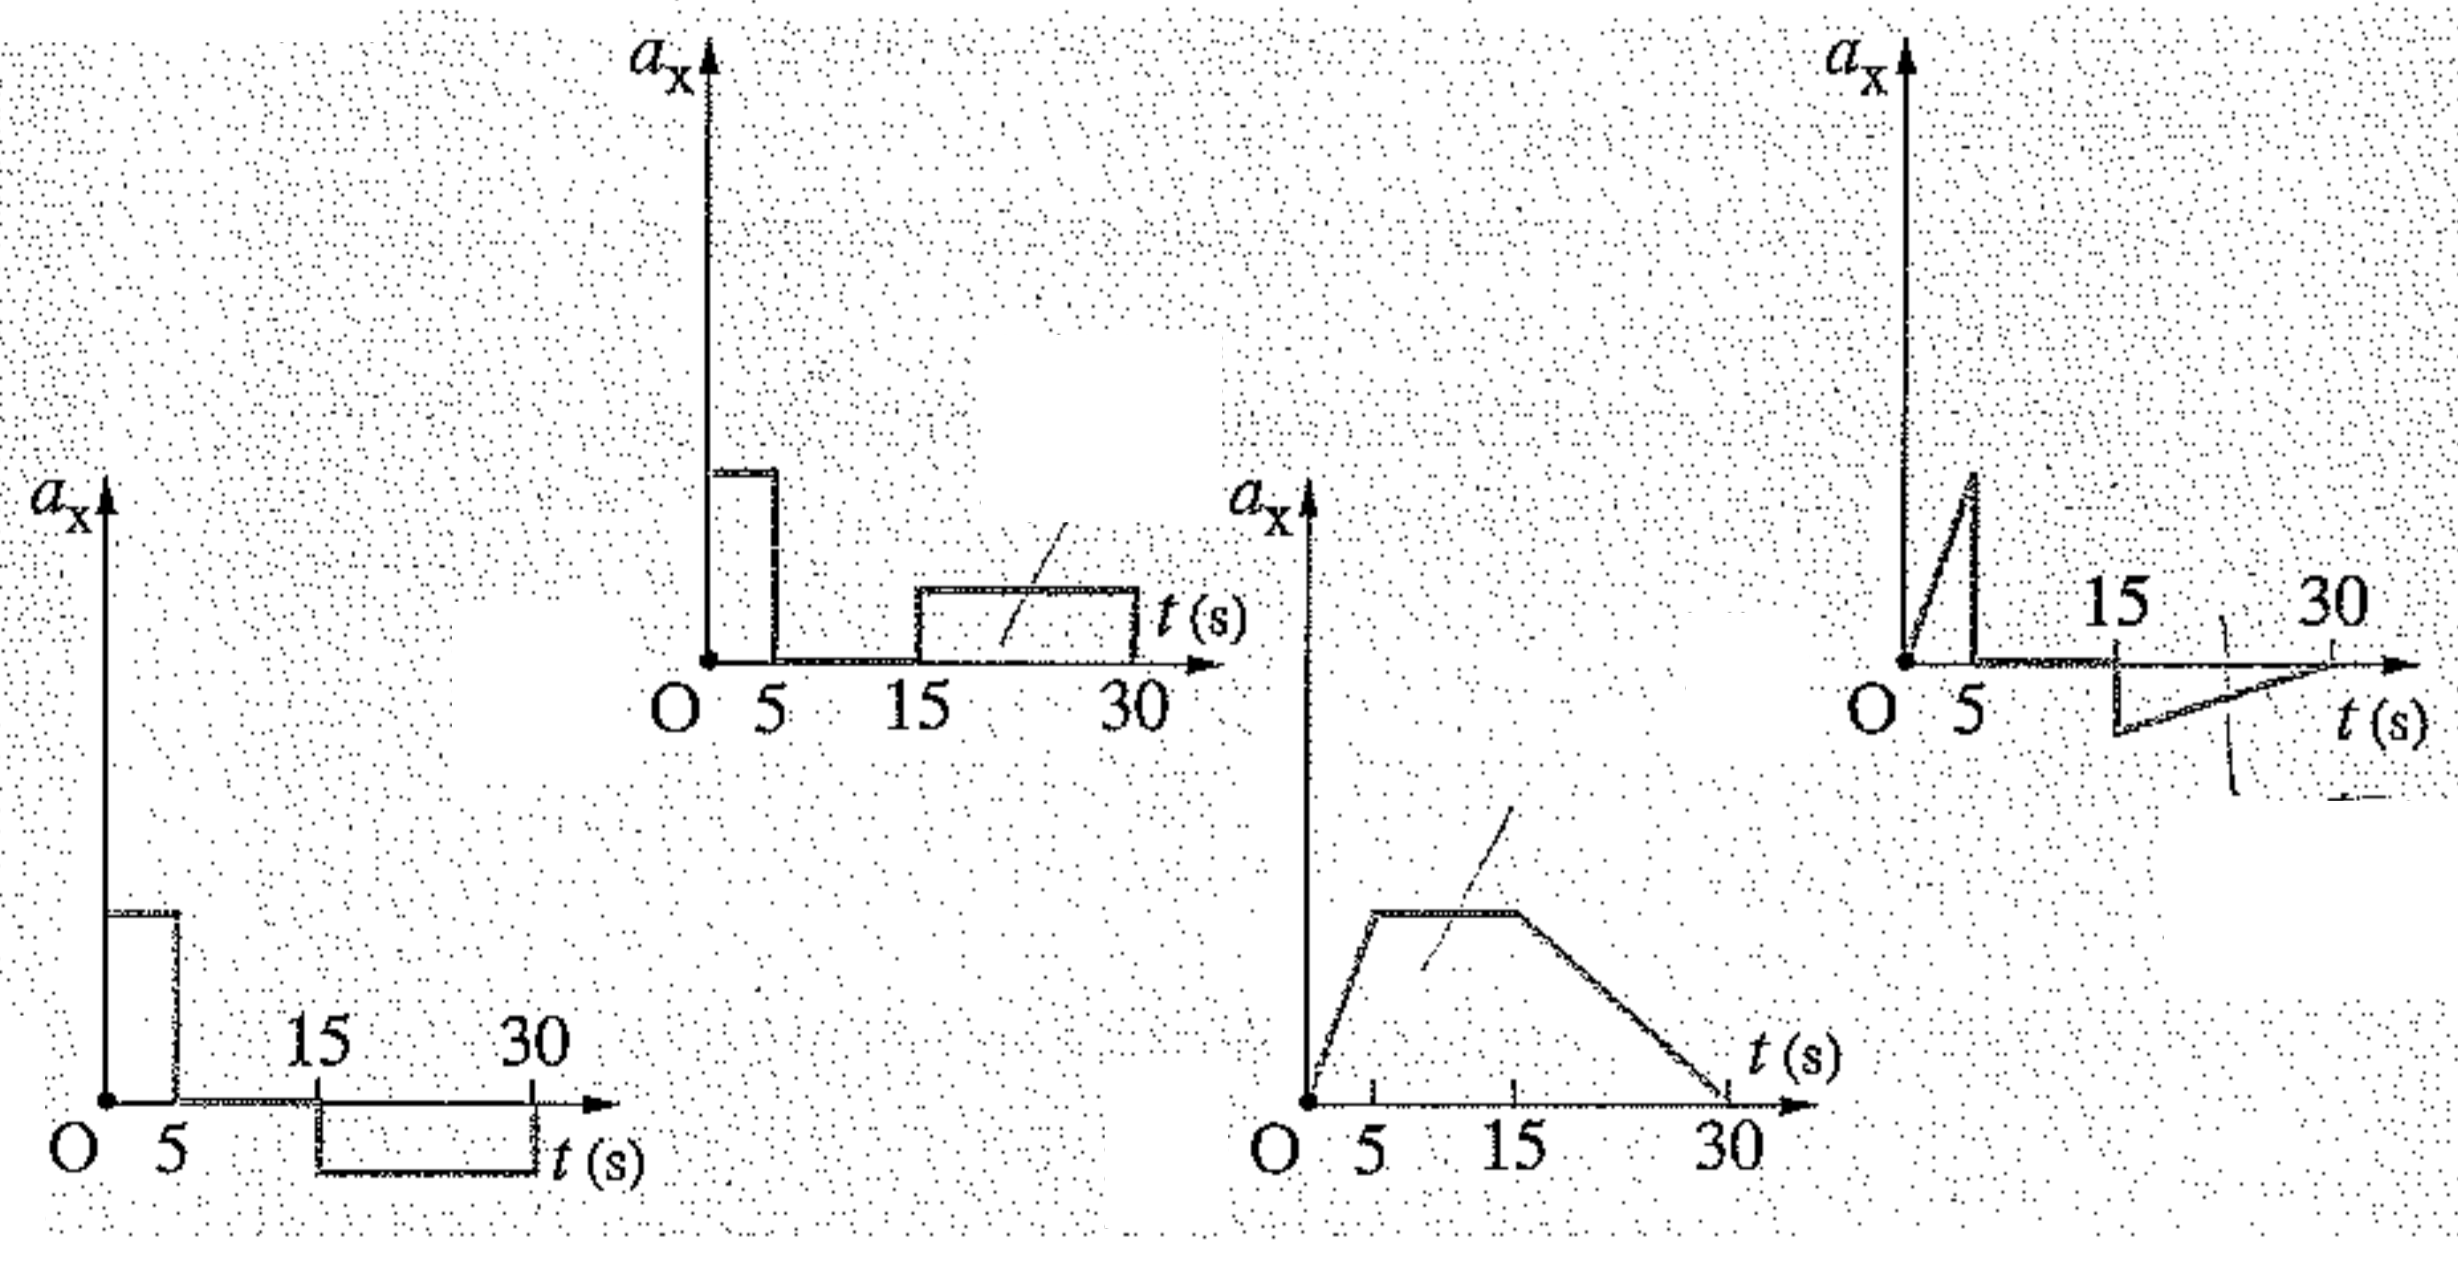
\includegraphics[width=0.93\textwidth]{snelheidsverloop_2}
% \end{image}

\begin{oplossing}
    Grafiek A 
\end{oplossing}
\end{question}
\end{exercise}



% Bron Serway 4yh edition oefening 77 chapter 2
\begin{exercise}
    ($\ast\ast\ast$) Maggie en Jennifer lopen de \SI{100}{m}. Beiden doen ze er exact \SI{10.2}{\second} over. 
    Met een eenparige versnelling bereikt Maggie na \SI{2}{\second} haar maximale snelheid, Jennifer doet dat na \SI{3}{s}. 
    Hun maximale snelheden houden ze aan voor de rest van de wedstrijd.
    \begin{question} Wat zijn hun maximale snelheden?                 
    \begin{oplossing} 
        $v_1=\frac{2x_2}{2t_2-t_1}$ 
    \end{oplossing} 
    \end{question}
    \begin{question} Wat is de versnelling van iedere sprinter?
    \begin{oplossing} 
        $a=\frac{2x_2}{(2t_2-t_1)t_1}$  
    \end{oplossing} 
    \end{question}
    \begin{question} Wie heeft er voorsprong na \SI{6}{s}, en hoeveel? 
    \begin{oplossing} $x_M-x_J=\frac{2x_2}{2t_2-t_{1,M}}(t-\frac{t_{1,M}}{2})-\frac{2x_2}{2t_2-t_{1,J}}(t-\frac{t_{1,J}}{2})$ 

        % ERROR: PDF OK; GEEN HTML VAN ONDERSTAANDE IMAGE 
        % \begin{image}
        %     \begin{tikzpicture}[yscale=0.5]
        %         \draw[->] (0,0) -- (14,0) node[right] {$t$ (s)};
        %         \draw[->] (0,0) -- (0,13) node[above] {$v$ (m/s)};
                
        %         \draw[dashed] (3,0) -- (3,12);
        %         \draw[dashed] (12,0) -- (12,12);
                
        %         \foreach \x in {0,3,12}
        %             \draw (\x,0) -- (\x,-0.2) node[below] {\x};
                
        %         \draw[thick] (0,0) -- (3,12) -- (12,12);
        %     \end{tikzpicture}
        % \end{image}
        % \captionof{figure}{Snelheidsgrafiek van Jennifer}
        % 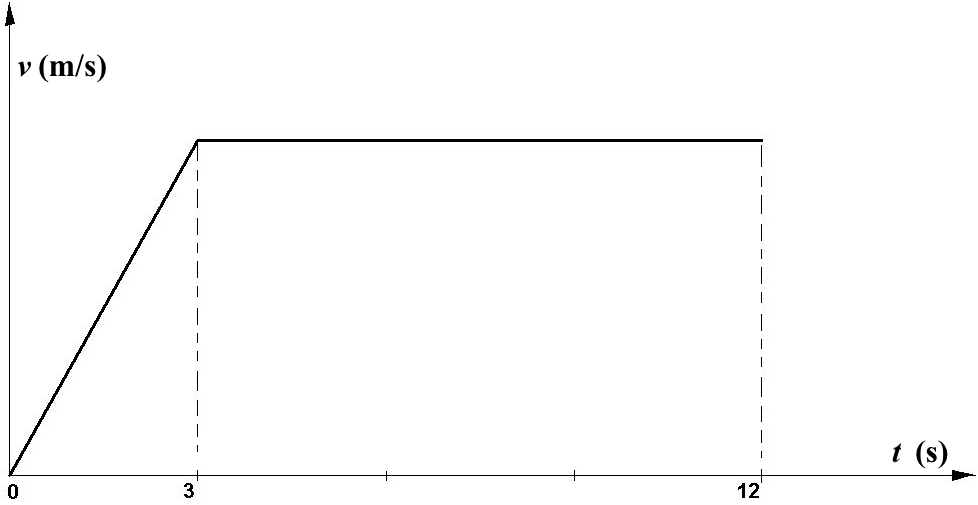
\includegraphics[width=0.5\textwidth]{sprinter}
    \end{oplossing} 
    \end{question}
\end{exercise}


\begin{exercise}
    Een auto die \SI{90}{\kilo\meter\per\hour} rijdt, ligt \SI{100}{m} achter op een vrachtwagen die \SI{75}{\kilo\meter\per\hour} rijdt. Hoeveel tijd kost het de auto om de vrachtwagen in te halen? 
    \begin{oplossing}
    Er is gegeven dat 
    \begin{itemize}
        \item \(V_A = \SI{25}{\meter\per\second}\)
        \item \(x_{0,A} = 0\)
        \item \(V_B - \SI{20.8}{\meter\per\second}\)
        \item \(x_{0,B} = \SI{100}{\meter}\)
    \end{itemize}

    Beide auto's bewegegen volgens een ERB. We berekenen: 

    \[
    \begin{array}{rcl}
        x_A &=& x_B\\
        v_A t &=& x_{0,B} + v_B t \\
        v_A t - V_B t &=& x_{0,B} \Rightarrow t = \frac{x_{0,B}}{v_A - v_B} = \SI{24}{\second}
        
    \end{array}\]


        $t=\frac{x_0}{v_a-v_v}=24\rm\,s$
    \end{oplossing}
\end{exercise}

\begin{exercise}
    De snelheid van een trein verandert eenparig in 2 minuten van \SI{20}{\kilo\meter\per\hour} tot \SI{30}{\kilo\meter\per\hour}. De trein rijdt gedurende die tijd over een rechte spoorlijn.
    \begin{question} Bepaal de versnelling.   
    \begin{oplossing}
    Er is gegeven dat 
    \begin{itemize}
        \item \(\Delta t = \SI{120}{\second}\)
        \item \(v_0 = \SI{5, 56}{\meter\per\second}\)
        \item \(v_1 = \SI{8,33}{\meter\per\second}\)
        \item \(x_0 = 0\)
    
        Een eenvoudige berekening levert de versnelling: \(a = \frac{\Delta v}{\Delta t} = \SI{0,0231}{\meter\per\second\squared}\)
    \end{itemize}
    \end{oplossing} 
    \end{question}
    \begin{question} Bepaal de afstand die de trein heeft afgelegd gedurende deze 2 minuten. 
    \begin{oplossing}
    Invlullen in de plaatsfunctie levert: 
    \[
    x_1 = v_0 \Delta t + \frac{1}{2}a (\Delta t)^2 = \SI{833}{\meter}
    \]

    \begin{remark}
        Er is ook een andere methode: 
        \[
        \begin{array}{rcl}
            \overline{v} = \frac{\Delta x}{\Delta t} &=& \frac{v_0 + v_1}{2}\\ 
            &\Downarrow&\\
            \Delta x &=& \frac{v_0 + v_1}{2} \cdot \Delta t = \SI{833}{\meter}
            
        \end{array}
        \]
    \end{remark}
    \end{oplossing} 
    \end{question}
\end{exercise}

\begin{exercise}
    Een auto trekt in \SI{5,0}{s} op van \SI{10}{m/s} naar \SI{25}{m/s}. Wat was de versnelling in de veronderstelling dat de auto een EVRB ondergaat? Welke afstand legde de auto in deze periode af?
    \begin{oplossing}
        De versnelling vinden we via $a=\frac{v-v_0}{t-t_0}=\SI{3}{\meter\per\second\squared}$. Via de opmerking voor bovenstaande oefening reken je eenvoudig uit dat $x-x_0=\left(\frac{v_0+v}{2}\right)(t-t_0)=\SI{87.5}{\meter}$
    \end{oplossing}
\end{exercise}

\begin{exercise}
    Op een vliegdekschip worden vliegtuigen gekatapulteerd op een startbaan van \SI{25}{\meter}. 
    Een opstijgend vliegtuig doorloopt dat traject vanuit rust op \SI{1}{\second} tijd en dat op eenparig versnelde manier.

    Zoek zijn versnelling en de snelheid waarmee het de baan verlaat.
    \begin{oplossing}
        Er is gegeven dat
        \begin{itemize}
            \item \(\Delta x = \SI{25}{\meter}\)
            \item \(\Delta t = \SI{1}{\second}\)
            \item \(v_0 = 0\)
            \item \(x_0 = 0\)
        \end{itemize}

        De beweging is een EVRB. Door de gegeven beginwaarden te gebruiken vinden we: 
        \[
        \begin{array}{rcl}
            x &=& t + \frac{1}{2}at^2 \\ 
            &\Downarrow&\\
            \Delta x &=& \Delta x = \frac{1}{2}(\Delta t)^2 \\
            &\Downarrow&\\
            a &=& \frac{2\Delta x}{(\Delta t)^2} = \SI{50}{\meter\per\second\squared}
            
        \end{array}
        \]
    \end{oplossing}
\end{exercise}

\begin{exercise}
    Een auto trekt vanuit rust op tot \SI{100}{\kilo\meter\per\hour} in \SI{6,0}{s}. Als hij dat doet op een rechte baan met constante versnelling, welke afstand is er dan hiervoor nodig?
    \begin{oplossing}
        Er is gegeven dat 
        \begin{itemize}
            \item \(v_0 = 0\)
            \item \(v_1 = \SI{27,8}{\meter\per\second}\)
            \item \(\Delta t = \SI{6}{\second}\)
            \item \(x_0 = 0\)
        \end{itemize}
        Een rechtstreekse berekening levert: 
        \[
        \begin{array}{rcl}
            x&=& \frac{1}{2}a t^2 = \frac{1}{2}\frac{\Delta v}{\Delta t}t^2\\
            &\Downarrow&\\
            \Delta x &=& \frac{\Delta v \cdot (\Delta t)^2}{2\Delta t} = \frac{\Delta v \Delta t}{2} = \frac{(v_1 - v_2)\Delta t}{2} = \frac{v_1}{2} \delta t = \SI{83,3}{\meter}
            
        \end{array}
        \]
    \end{oplossing}
\end{exercise}


\begin{exercise}
    Een vliegtuig landt met een snelheid van \SI{100}{m/s}. Op de ladingsbaan heeft het een vertraging van \SI{5,0}{m/s^2}. Welke afstand heeft het vliegtuig nodig om tot stilstand te komen?
    \begin{oplossing}
        Er is gegeven dat: 
        \begin{itemize}
            \item \(v_0 = \SI{100}{\meter\per\second}\)
            \item \(a = \SI{-5}{\meter\per\second\squared}\)
            \item \(v_1 = 0\)
            \item \(x_0 = 0\)
        \end{itemize}
        Het vliegtuig beweegt volgens een EVRB. We hebben volgende bewegingsvergelijkingen: 
        
        \[\left\{
            \begin{array}{rcl}
            x&=& x_0 + v_0t+\frac{1}{2}at_1^2 \\
            v&=& v_0 + at
            \end{array}
        \right.
        \]
        Uit de snelheidsvergelijking halen we \(t_1 = \frac{-v_0}{a}\). Invullen in de eerste vergelijking levert: 
        \[
        \begin{array}{rcl}
            x_1 &=& v_0t_1 + \frac{1}{2}at_1^2\\
            &=& \frac{-v_0^2}{a} + \frac{av_0^2}{2a^2}\\
            &=& \frac{-v_0^2}{a} + \frac{v_0^2}{2a}\\
            &=& \frac{-v_0^2}{2a}\\
            &=& \SI{1000}{\meter}
        \end{array}
        \]
    \end{oplossing}
\end{exercise}

\begin{exercise}
    Een trein vertrekt uit een station en rijdt op een recht spoor met een eenparig versnelde beweging waarvan de versnelling \SI{0,50}{m/s^2} bedraagt. 
    Hoe groot is de afstand die de trein heeft afgelegd als zijn snelheid \SI{72,0}{\kilo\meter\per\hour} bedraagt?
    \begin{oplossing}
        Er is gegeven dat 
        \begin{itemize}
            \item \(v_0 = 0\)
            \item \(a = \SI{0.5}{\meter\per\second\squared} \) 
            \item \(v_1 = \SI{20}{\meter\per\second}\)
            \item \(x_0 = 0\)
        \end{itemize}
        
        De trein beweegt volgends een EVRB. Uit de snelheidsfunctie \(v_1 = v_0 +at\) halen we dat \(t_1 = \frac{v_1}{a}\). Deze gevonden \(t_1\) substitueren we in de plaatsfunctie: 
        \[
        \begin{array}{rcl}
            x1 &=& x_0 + v_0t_1 + \frac{1}{2}at_1^2\\
            &=& \frac{1}{2}a (\frac{v_1}{a})^2 \\
            &=& \frac{v_1^2}{2a}\\
            &=& \SI{400}{\meter}

            
        \end{array}\]
    \end{oplossing}
\end{exercise}

\begin{exercise}
    Twee personen A en B voeren op dezelfde rechte en vanuit dezelfde beginstand een eenparige beweging uit. 
    A vertrekt \SI{100}{s} eerder dan B. Met een snelheid die dubbel zo groot is als die van A haalt B, op \SI{400}{m} van het vertrekpunt, A in. 
    Bereken beide snelheden en stel ze grafisch voor.

    \begin{oplossing}
    Er is gegeven dat 
    \begin{itemize}
        \item \(\SI{1}{\meter}\)
        \item \(t_{0,B} = \SI{100}{\second}\)
        \item \(v_b = 2v_a\)
        \item \(x = \SI{400}{\meter}\)
    \end{itemize}
    % \item[gegeven]$x_0=1,00\cdot10^3\rm\,m$\newline$t_0=100\rm\,s$\newline$v_b=-2v_a$\newline$x=400\rm\,m$
    % \item[gevraagd]$v_a$, $v_b$
    % \item[oplossing]De bewegingsvergelijkingen voor A en B worden gegeven door:

    % \begin{eqnarray}
    % A:\qquad x&=&v_at \label{verg A}\\
    % B:\qquad x&=&x_0+v_b(t-t_0)\nonumber\\
    % &=&x_0-2v_a(t-t_0) \label{verg B}
    % \end{eqnarray}

    \[
    \left\{
        \begin{array}{rcl}
            x(t) &=&v_at\\
            x(t) &=&x_0+v_b(t-t_0) = x_0-2v_a(t-t_0)
        \end{array}
    \right.
    \]

    De grafiek van beide functies ziet er als volgt uit:
    
    \begin{image}[0.5\textwidth]
        \begin{tikzpicture}
            \draw (-0.5, 0) -- (5,0) node[right]{$t$};
            \draw (0, -0.5) -- (0,5) node[above]{$x$};

            \coordinate (O)  at (0, 0); 
            \coordinate (A2) at (5, 5); 
            \coordinate (B1) at (1.5, 0); 
            \coordinate (B2) at (4, 5); 

            \draw[name path=lijn1] (0,0) -- (A2) node[pos=0.9, right]{\(A\)};
            \draw[name path=lijn2] (B1) -- (B2) node[pos=0, below]{\(\SI{100}{\second}\)} node[pos=0.9, above left]{\(B\)};

            \path[name intersections={of=lijn1 and lijn2}];

            \fill[red] (intersection-1) circle (3pt) node{\(S\)};


            \draw[dashed] (intersection-1) -- (intersection-1 |- O) node[below]{\(\Delta t\)};
            \draw[dashed] (intersection-1) -- (intersection-1 -| O) node[left]{\(\SI{400}{\meter}\)};
        \end{tikzpicture}
    \end{image}

    Als we voor $x$ de ontmoetingsplaats van \SI{400}{m} nemen, hebben we twee vergelijkingen en twee onbekenden $t$, $v_a$. 
    Dit kunnen we oplossen door een variabele te substitueren. We nemen de tijd, $\Leftrightarrow t=\frac{x}{v_a}$ en substitueren deze in vergelijking:

    \[
    \begin{array}{rcl}
    x&=&x_0-2v_a(t-t_0)\\
    &=&x_0-2v_a\left(\frac{x}{v_a}-t_0\right)\\
    &\Updownarrow&\\
    v_a&=&\frac{3x-x_0}{2t_0}=\SI{1}{\meter\per\second}
    \end{array}
    \]

    En de snelheid van B:

    \[
    v_b=-2v_a=\frac{x_0-3x}{t_0}= \SI{-2}{\meter\per\second}
    \]

    \end{oplossing}

\end{exercise}

\begin{exercise}
    Aan het begin van een rechte landingsbaan, start een vliegtuig vanuit rust en versnelt met een constante versnelling langs de grond alvorens op te stijgen. 
    Het legt \SI{600}{m} af in \SI{12}{s}. 
    Bepaal de versnelling, de snelheid na \SI{12}{s} en de afstand afgelegd gedurende de twaalfde seconde.

    \begin{oplossing}
    Er is gegeven dat 
    \begin{itemize}
        \item \(v_0 = 0\)
        \item \(x_0 = 0\)
        \item \(x_1 = \SI{600}{\meter}\)
        \item \(t_1 = \SI{12}{\second}\)
    \end{itemize}

    Het vliegtuig beweegt volgens een EVRB waarvoor 
    \[
    \begin{array}{rcl}
        x_1 &=& \frac{1}{2}at_1^2\\
        & \Downarrow & \\
        a &=& \frac{2x_1}{t_1^2} = \SI{8,33}{\meter\per\second\squared}
    \end{array}\]

    De snelheid vinden we door deze bekomen \(t_1\) te substitueren in de snelheidsfunctie: 

    \[
    v_1 = v_0 + at = \SI{100}{\meter\per\second}
    \]

    De afgelegde weg is gelijk aan 

    \[
    \begin{array}{rcl}
        \Delta x &=& x_1 - x_2 \\
        &=& x_1 - \frac{1}{2}at_2^2 \\
        &=& \SI{600}{\meter} - \SI{500}{\meter} \\
        &=& \SI{96}{\meter} \\

    
    \end{array}\]
    \end{oplossing}
\end{exercise}


% oefeningen ingevoegd die in de theorie stond 
\begin{exercise}

    Een auto die $\SI{60}{km/h}$ rijdt, raakt een boom; de voorkant van de auto wordt in elkaar gedrukt en de bestuurder komt na $\SI{70}{cm}$ tot stilstand. Welke gemiddelde vertraging onderging de bestuurder tijdens de botsing?% Druk je antwoord uit in $g$, waarbij $g=\SI{9,81}{m/s^2}$.
    \begin{oplossing} 
    Er is gegeven dat 
    \begin{itemize}
        \item \( v_0 = \SI{16,7}{\meter\per\second}\)
        \item \(v_1 = 0\)
        \item \(\Delta x = \SI{0.7}{\meter}\)
    \end{itemize}
    Om de (constante) vertraging te vinden, hebben we de snelheidsverandering en de benodigde tijd nodig. 
    De verandering in snelheid kennen we; de eindsnelheid van de auto moet nul worden maar de duur is niet onmiddellijk gegeven. 
    Omdat de eindsnelheid nul is, kunnen we wel uit de snelheidsvergelijking van een eenparig veranderlijke beweging een \textit{uitdrukking} vinden voor die tijd die we vervolgens kunnen substitueren in de plaatsvergelijking. De enige onbekende is dan de gezochte versnelling.\footnote{M.b.v. de formule $\overline{v}=\frac{v_0+v}{2}$ voor de gemiddelde snelheid en de definitie voor de gemiddelde snelheid $\overline{v}=\frac{\Delta x}{\Delta t}$ is het antwoord sneller te vinden. Ga maar na \ldots}

    Uit $v(t)=0$ of $0=v_0+at$ halen we een uitdrukking voor de tijd die nodig is om tot stilstand te komen:
    \[
    t =-\frac{v_0}{a}
    \]

    Substitutie van deze tijd in de plaatsfunctie levert:

    \[
    \begin{array}{rcl}
    x&=&v_0t+\frac{1}{2}at^2\\
    &=&v_0\left(-\frac{v_0}{a}\right)+\frac{1}{2}a\left(-\frac{v_0}{a}\right)^2\\
    %&=&-\frac{v_0^2}{a}+\frac{v_0^2}{2a}\\
    &=&-\frac{v_0^2}{2a}\\
    \end{array}
    \]
    De versnelling is dan gelijk aan:
    \[
    a = -\frac{v_0^2}{2x}
    \]

    Invullen van de gegevens levert $a=\SI{-198}{m/s^2}$.%, wat gelijk is aan $20g$.
    \end{oplossing}
    \end{exercise}
    
\end{document}
